\documentclass[ms,electronic,twosidetoc,letterpaper,chaptercenter,parttop,lol,lof,lot]{byumsphd}
\usepackage{slatex}
\usepackage{graphicx}
\usepackage[
    bookmarks=true,
    bookmarksnumbered=true,
    breaklinks=false,
    raiselinks=true,
    pdfborder={0 0 0},
    colorlinks=false,
    plainpages=false,
    ]{hyperref}

\usepackage[all]{hypcap}
\usepackage[numbers,sort&compress]{natbib}
\usepackage{hypernat}

\newcommand{\Title}{Autocompletion for the Rest of Us}
\newcommand{\Author}{Nick Shelley}
\newcommand{\GraduationMonth}{August}
\newcommand{\GraduationYear}{2014}

\hypersetup{%
    pdftitle=\Title,%
    pdfauthor=\Author,%
    pdfsubject={Masters Thesis, BYU CS Department: %
                Degree Granted \GraduationMonth~\GraduationYear, Document Created \today},%
    pdfkeywords={BYU, thesis, dissertation, LaTeX},%
}

\newcommand{\ItemSep}{\itemsep 0pt}
\let\oldenum=\enumerate
\renewcommand{\enumerate}{\oldenum \ItemSep}
\let\olditem=\itemize
\renewcommand{\itemize}{\olditem \ItemSep}
\let\olddesc=\description
\renewcommand{\description}{\olddesc \ItemSep}

\title{\Title}
\author{\Author}

\committeechair{Jay~McCarthy}
\committeemembera{Bryan~Morse}
\committeememberb{Dennis~Ng}

\monthgraduated{\GraduationMonth}
\yeargraduated{\GraduationYear}
\yearcopyrighted{\GraduationYear}

\documentabstract{%
Code completion systems act both as a way to decrease typing and as a way to easily access documentation, both implicit and explicit.
The former is typically done by completing known variable or function names, while the latter is done by providing a list of possible completions or by providing convenient views of or access to documentation.
Because static type information makes these goals possible and feasible for qualifying languages, many improvements to completion systems are focused on improving the order of results or trimming less-valuable results.
It follows that almost all validation techniques for this work have focused on proving how well a completion system can put a desired result at the top of the list.
However, because of the lack of static type information in dynamically-typed languages, achieving the aforementioned goals is much harder, and many of the completion suggestions may even result in compile-time or runtime crashes.
Unfortunately, of the work done on creating completers for these languages, little validation work has been done, making it hard to determine what improvements can be made.
This thesis will provide two validation techniques that will provide information both on how well completion suggestions are ordered and also which completion suggestions result in errors.
This information will be used to guide the development and evolution of a completion system for the Racket programming language.
}

\documentkeywords{%
    code completion, auto-complete, autocomplete
}

\acknowledgments{%
    Thanks to Dr. McCarthy for his support and patience.
}

\department{Computer~Science}
\graduatecoordinator{Quinn~Snell}
\collegedean{Thomas~W.~Sederberg}
\collegedeantitle{Associate~Dean}

% Customize the name of the Table of Contents section.
\renewcommand\contentsname{Table of Contents}

% Remove all widows an orphans.  This is not normally recommended, but in a
% paper dissertation there is no reasonable way around it; you can't exactly
% rewrite already-published content to fix the problem.
\clubpenalty 10000
\widowpenalty 10000

% Allow pages to have extra blank space at the bottom in order to accommodate
% removal of widows and orphans.
\raggedbottom

% Produce nicely formatted paragraphs. There is nothing additional to do.  In
% case you get some problems, surround your text with
% \begin{sloppy} ... \end{sloppy}. If that does not work, try
% \microtypesetup{protrusion=false} ... \microtypesetup{protrusion=true}
\usepackage{microtype}

\begin{document}

% Produce the preamble
\microtypesetup{protrusion=false}
\maketitle
\microtypesetup{protrusion=true}

\chapter{Introduction}

\paragraph{Thesis Statement} For auto-completers for languages like Racket, textual and structural heuristics perform better than macro heuristics and analyses, and when combined perform better than either alone.
Macro heuristics perform almost equivalent to macro analyses, and structural heuristic performance varies depending on editing mode.

\paragraph{} The main purpose of autocompletion is to improve programmer productivity.
This has mainly been accomplished in two ways.
The first way is to reduce typing by predicting which token(s) should be inserted at a given position, sometimes replacing the partially-typed token.
Incidentally, this also encourages more descriptive variable names since longer names can be completed automatically.
The second way is to provide convenient documentation to the programmer.
For example, a list of currently valid (i.e. in scope, correctly typed, etc.) substitutions may be provided given the current cursor position.
Also, a function's signature and purpose can be displayed next to the typed function name.
This thesis focuses on the first way of completing textual tokens rather than providing convenient documentation.

Static type information makes it relatively simple for completions systems for such languages to filter out invalid results.
However, because type information is not known statically in other languages, it is possible and easy to suggest tokens that may result in runtime errors and others that may not even compile.
Because static type information makes it possible to suggest completions with high assurance of being valid, research and work on completers for such languages have focused mainly on presenting these valid results in a way that is more useful to the programmer.
For instance, instead of giving all valid results in alphabetical order, results can be omitted or promoted closer to the top of the list based on context, type, or analysis of previous code.
Therefore, validation systems have mainly focused on how well a desired token makes it in the top N suggestions.

Other features that make autocompletion hard for certain languages include first-class functions and powerful macro systems.
I will now discuss the challenges these features pose in detail.

% set up slatex stuff
\setkeyword{racket require for-syntax provide}

\section{Dynamic Typing}

Dynamically typed languages do the majority of their type checking at run-time as opposed to compile-time.
In dynamic typing, values have types but variables do not.
A variable can thus refer to any value of any type at any time.

Because a variable's type can change at any time in the program, the type information can't be used to filter which variables can appear in which contexts.
For example, consider the incomplete programs in Figure~\ref{fig:dynamic-type}.
Should an auto-completer give the parameter \scheme{a} as an option to fill the hole in \texttt{dynamic-parameter.rkt}?
With the call \scheme{(add2 5)}, the program would have a meaningful result.
However, with the call \scheme{(add2 #t)}, there would be a run-time error.
Since the auto-completer can't know at compile-time what types of values the parameter \scheme{a} can possibly hold, it cannot know whether it is correct to include it in the auto-complete list.

As another example, consider the two holes in \texttt{dynamic-return-value.rkt}.
The auto-completer needs to make a decision about whether or not to include \scheme{num} in the list of suggestions.
If \scheme{num} filled the first hole, the number \scheme{10} would be inserted and the result of the program would be \scheme{15}.
However, if \scheme{num} filled the second hole, the string \scheme{"hi"} would be inserted and a run-time error would occur.
Although it is easy for us as humans to look at these two function calls and know what they will return, it is hard for a computer to do so without running the program first.
We can also imagine more complicated functions which would be hard for both humans and computers to analyze.
Since the auto-completer can't statically know what type a function will return, it cannot know whether it is correct to include the result of a function in the auto-complete list.

\begin{figure*}[t]
\hrule
\centering
\renewcommand{\arraystretch}{2}
\begin{tabular}{c@{\hspace{0.2\linewidth}}c}
\texttt{dynamic-parameter.rkt}
&
\texttt{dynamic-return-value.rkt}
\\
\begin{minipage}[t]{\linewidth}
\begin{schemedisplay}
#lang racket
(define (add2 a)
  (+ [ ] 2))
\end{schemedisplay}
\end{minipage}
&
\begin{minipage}[t]{\linewidth}
\begin{schemedisplay}
#lang racket
(define (return-something a)
  (if (< a 5) 10 "hi"))

(define num (return-something 2))
(+ [ ] 5)
(set! num (return-something 8))
(+ [ ] 5)
\end{schemedisplay}
\end{minipage}
\\
\end{tabular}
\vspace{0.5cm}
\hrule
\caption{Problems with Dynamic Typing}
\label{fig:dynamic-type}
\end{figure*}

\section{First-class Functions}

Support for first-class functions means functions can be passed around as values.
Coupled with the dynamic typing problem, first-class functions make it impossible to know which bindings are functions and which aren't.
Ideally, if an auto-completer is invoked where it makes sense to call a function (such as after an opening parenthesis), only functions should appear in the list of suggestions.
However, because we can't know which bindings are functions, we must consider all bindings.
For example, the program \texttt{function-parameter.rkt} in Figure~\ref{fig:first-class-functions} contains two holes, one where a boolean should go, and another where a function should go.
Because passing \scheme{+} to \scheme{fun} is just as valid as passing \scheme{#t} or \scheme{3}, we can't know if it is correct to include the parameter \scheme{f} in either of those holes.

Even if we could know or assume that a function is being called, we cannot know which function a variable is bound to.
This makes bringing up information about the function, such as a parameter list, impossible.
For example, the program \texttt{function-return.rkt} in the same figure contains two holes.
In the first instance we would want the auto-completer to bring up the possible parameters to the \scheme{+} function that will be returned, which are \scheme{z ...}.
In the second instance we would want the auto-completer to bring up \scheme{make-vector}'s possible parameters, which are \scheme{size [v]}.
However, because we don't know what function will be returned, we cannot bring up the correct parameters. 

\begin{figure*}[t]
\hrule
\centering
\renewcommand{\arraystretch}{2}
\begin{tabular}{c@{\hspace{0.2\linewidth}}c}
\texttt{function-parameter.rkt}
&
\texttt{function-return.rkt}
\\
\begin{minipage}[t]{\linewidth}
\begin{schemedisplay}
#lang racket
(define (fun f)
  (when [ ] ([ ] 3 2))
\end{schemedisplay}
\end{minipage}
&
\begin{minipage}[t]{\linewidth}
\begin{schemedisplay}
#lang racket
(define (return-fun a)
  (if (< a 5) + make-vector))

((return-fun 2) [ ])
((return-fun 7) [ ])
\end{schemedisplay}
\end{minipage}
\\
\end{tabular}
\vspace{0.5cm}
\hrule
\caption{Problems with First-class Functions}
\label{fig:first-class-functions}
\end{figure*}

\section{Powerful Macro System}

Racket macros are essentially an API to add compiler extensions.
All macros compile down to a small set of core language features, potentially going through intermediate transformations when other macros are used in macro definitions.
Most of the features available in Racket are macro definitions.
For example, the \scheme{and} and \scheme{or} constructs are actually macros that compile to the core \scheme{let} and \scheme{if} constructs.
Macros such as \scheme{or} can be used to define other macros, which can be used to define yet more macros.
A program is said to be fully expanded when all macros have been recursively transformed until only core language constructs remain.

Syntax objects are an important part of the Racket macro system.
Syntax objects basically wrap source code with lexical and location information.
For example, a syntax object for the symbol \scheme{x} could have lexical information describing which bindings are visible to \scheme{x}.

Racket macros are transformers that take a syntax object and return a syntax object, or in other words, they take source code and return source code.
The syntax object returned can do anything it wants with the syntax object passed in, or it could ignore its input and return an arbitrary syntax object.
In other words, Racket macros can do arbitrary things to the program.

Figure~\ref{fig:macros} shows macros that can cause problems for an auto-completer.
In \texttt{binding.rkt}, the \scheme{not-define} macro introduces a binding for the variable \scheme{x}, breaking its promise not to define anything.
It does this by extracting the value from the syntax object passed in and creating a new syntax object that defines \scheme{x} as this value.
However, by examining the program, an auto-completer has no indication that \scheme{x} has been defined anywhere.
In particular, at the hole in the \scheme{+} application in \texttt{binding.rkt}, the auto-completer is not aware that \scheme{x} is an available binding.

In \texttt{context.rkt}, \scheme{x} is bound to \scheme{5} within the \scheme{let}.
By examining the source code, an auto-completer could give \scheme{x} as an option at the hole within the \scheme{let}.
However, in this case the addition expression is passed to the \scheme{f} macro.
This macro essentially replaces the context of the expression passed in with the context of \scheme{anchor}.
Since \scheme{anchor} was defined at the top-level, the expression returned from \scheme{f} will only have access to top-level bindings.
This can cause two problems.
As we see in \texttt{context.rkt}, \scheme{x} is bound to \scheme{#f} at the top level, so filling the hole with \scheme{x} would cause a run-time error to occur.
Even an auto-completer that was smart enough to get around the dynamic typing problem by only including bindings of the correct type would be fooled by this scenario.
Thus the first problem is essentially a complication of the dynamic typing problem.
However, if we remove the definition of \scheme{x} at the top-level, then there would be no binding for \scheme{x} available to the expression, which would cause a compile-time error.

\begin{figure*}[t]
\hrule
\centering
\renewcommand{\arraystretch}{2}
\begin{tabular}{c@{\hspace{0.2\linewidth}}c}
\texttt{binding.rkt}
&
\texttt{context.rkt}
\\
\begin{minipage}[t]{\linewidth}
\begin{schemedisplay}
#lang racket
(define-syntax (not-define stx)
  (syntax-case stx ()
    [(_ v)
     (with-syntax ([id (datum->syntax stx 'x)])
       (syntax
        (define id v)))]))

(not-define 6)
(+ [ ] 2)
\end{schemedisplay}
\end{minipage}
&
\begin{minipage}[t]{\linewidth}
\begin{schemedisplay}
#lang racket
(require (for-syntax syntax/strip-context))
(define-for-syntax anchor #'here)
(define-syntax (f stx)
  (syntax-case stx ()
    [(_ e)
     (replace-context anchor #'e)]))

(define x #f)
(let ([x 5])
  (f (+ [ ] 2)))
\end{schemedisplay}
\end{minipage}
\\
\end{tabular}
\vspace{0.5cm}
\hrule
\caption{Problems with Macros}
\label{fig:macros}
\end{figure*}

\paragraph{} As shown, these language features make it especially hard to implement completion systems for such languages.
Because of this, work in this area has focused on providing suggestions in a similar way to static completers.
Because validation efforts for such completers are minimum, improvements to such systems relies on user complaints, and implementing new systems correctly is hard at best.

\chapter{Related Work}

Some commercial and research completion systems have been implemented for dynamically-typed languages such as PHP and JavaScript \cite{Mapping, Semantic, Vs.php, JScript}.
These systems use knowledge about the structure of the language to complete common constructs such as functions, objects, and variables.
Dynamic information is either ignored or else semantic analysis and type inference is used to statically determine as much information as possible.
None of these systems provide or document any sort of testing or validation framework.

For traditional completion systems, many possible improvements have been explored over the traditional alphabetical sorting of all possible suggestions.
The jungloid mining approach~\cite{Jungloid} uses intimate knowledge about the Java type system, library and API functions, example code, and the current context of the program to suggest ways to get from one type to another type through intermediate steps.
Bcc~\cite{BCC} sorts by Java type starting with methods provided from the declared type and then up the type hierarchy until the base Object class.
It also allows for custom filters to be specified by the programmer.
The abbreviated input approach\cite{Abbreviated} takes abbreviated input instead of prefixes and uses a hidden Markov model to determine what was meant.
For example, the expression \texttt{ch.opn(n)} would turn into \texttt{chooser.showOpenDialog(null)}.
The program history approach~\cite{History} tracks all changes to the codebase and prioritizes suggestions based on how recently methods and objects have been changed.
The examples approach~\cite{Examples} uses existing code (such as the Eclipse code base) as training data to implement three different completion systems.
The first orders suggestions based on how frequently they are used.
The second uses limited context information to create association rules that govern suggestion order.
For instance, one rule might be that after objects are created, suggest setters on those objects.
The third gathers context and uses a modification of the k-nearest-neighbor algorithm to order suggestions based on the nearest snippets found in the training data.

Most validation techniques ran their systems on modified existing code and ranked the results in some way.
The authors of the abbreviated input paper~\cite{Abbreviated} ran their system on 3000 lines of code from 6 open source projects that were turned into acronym-like abbreviations.
They measured how many lines could be completed and how many of those were in the top-N (i.e. top-1 or top-5) suggested completions.
Hou and Pletcher~\cite{Towards} ran their completion system at every Swing method in several open source projects.
They ranked how high in the suggestions list the actual method appeared and added all rankings together to get an overall ranking for the system.
The program history paper~\cite{History} ran their completion system between every recorded change operation (defined as a change in the AST) on a project of theirs called SpyWare.
They then recorded what percentage of actual methods were in the top-N suggestions.
Lastly, the examples paper~\cite{Examples} used the Eclipse code base and randomly split the code into 90\% training data and 10\% test data.
They then took out half of the Swing method calls in the test data and ran their completion system in each hole.
They measured recall, which is how often a used method was in the suggestion list, and precision, which is what fraction of suggested methods were actually used.
They then combined these two measures into an F1-measure to give an overall grade to a system.

Several papers related to code completion but not immediately relavent to this thesis are described here.
One paper uses a database of API usage patterns to improve completion~\cite{Graph}.
Another allows developers to customize inline documentation~\cite{Active}.
Calcite~\cite{Calcite} suggests popular ways to instantiate a given class or interface.
Similarly, another paper provides suggestions based on current structural context~\cite{StructuralContext}.
Another paper explores the effects of sorting, filtering, and grouping~\cite{SortFilter}.
Vertical Code Completion~\cite{Vertical} uses data mining to extract and suggest code patterns.
One paper offers suggestions based on partial expressions written by programmers~\cite{Partial}.
Finally, Automatic method completion~\cite{Automatic} attempts to take completion beyond names to function bodies as well.

The lack of testing done on dynamic auto-completers helped emphasize the need for a validation system for such languages.
The testing done on most static auto-completers inspired the use of random testing on existing code.
The metrics they used are all similar and helped define metrics in a way that works best for such validation systems.
Lastly, although a lot of improvements were type-system specific, some methods inspired ideas for completion approximation methods implemented as part of this thesis.

\chapter{Implementation}

Very little formal testing has been done in the area of code completion for languages like Racket, leaving a need for formal testing in this area.
There are several viable solutions to the testing problem.
One set of methods includes performing user studies or collecting user feedback from using the product.
Another set of methods includes using existing source code as a baseline for correct completer results.
This set could include seeing where existing source tokens are ordered in a list of potential completer results as well as checking whether completer results cause a program to fail.

We implement the latter set of methods for several reasons.
First, methods involving user testing or feedback require products to be in a workable state, making continuous testing feedback more difficult.
Second, these methods are more costly and time consuming than the latter methods.
Last, much more is known in the literature about the first set of methods, whereas little has been done to show how automated testing can help completers for languages such as Racket, thus making our work more of a contribution to the field.

\section{Existing Source}

We choose several large real-world Racket packages as the existing source to use in our testing framework.
Frog is a static website generator, mainly used for generating and updating blogs.
Marketplace is a network-aware programming language that handles many problems inherent with distributed programming.
PFDS is an implementation of many purely functional data structures written in Typed Racket.

In order to test against existing source, the source file must be tokenized.
One way to do this is just to delimit on whitespace.
However, since it is uncommon for data such as numbers and strings to use code completion, we use the language grammar to only test valid identifiers.

Since testing every token of every source file can take a very long time when the amount of source code is large, we use randomized testing to save time while still collecting representative data.
To do this, we collect all of the tokens from a file, excluding data such as strings and numbers. 
We then randomly choose a percentage of those tokens to test against.

There are many ways a source file can be modified.
One way is to create a new source file and begin filling it with code.
Another is to take an existing source file and either add more source or modify the existing source.
We predicted that the second case is easier to complete against because there was more information.
We weren't surprised to find that this was true.
In order to use existing source as test data, the original source must be modified to remove one or more tokens at which point the completer will be run.
We choose two simple ways to modify the source.
The first way is to truncate the source file after the chosen identifier.
This represents writing new source code because if the file were being written from scratch, there would be nothing after the token.
The second way is to simply remove the token from the source file, which represents modifying or maintaining existing source code.

\section{Testing Framework}

There are two main ways that existing source can be used to verify completion results.
The first is to check the occurrence and rank of existing source tokens.
This requires the assumption that the programmer wrote what they intended.
The second is to check that completion suggestions do not break the program.
This requires the assumption that existing source can be compiled and run without errors.
We implement both methods of verification in our automated testing framework.

\subsection*{Ranker}

For a given token in a source file, the ranker will modify the file at that position, either by removing or truncating as described above, and then invoke an auto-completer to get a list of completion results.
It then compares the list of results to the original token, which represents the programmer's intent.
If the original token is found in the first $n$ results (a configurable number), its rank is recorded.
It is also noted whether the original token is found later in the list or not at all.
In the graphs and data presented, $n = 5$.

This method of testing completion results allows changes affecting the number and location of results to be checked quantifiably and consistently.

\subsection*{Checker}

Similar to the ranker, the checker asks an auto-completer for a list of completions from a modified source file.
However, instead of checking against the original token, the original token is replaced by one of the completion results, and the resulting program is compiled and run.
If the program runs to completion, the completion result is recorded as a success.
If the program fails to compile or terminates for any reason, the type of error is recorded.

This method allows auto-completers to test how top completion results fail for different methods of completion.
With this information, targeted changes can help reduce certain types of failures.

\chapter{Verification}

The best way to verify a testing framework is to use it to test existing implementations and analyze the results, making sure they are helpful and make sense.
We create our own set of completer implementations to ensure that the testing framework is exercised in full and because we don't have access to existing implementations for Racket.

We implement two main categories of completion.
The first category is textual analysis.
This category takes as its primary input the source text from a single source file.
Methods in this category may use knowledge about the language to improve results.
The second category attempts to solve or mitigate the problems presented to completion systems due to the existence of a powerful macro system, as described above.

\section{Method Descriptions}

\subsection{Textual Heuristics}

One obvious source of potential completion options if from the source file itself.
We estimate that many correct completions can be pulled from the source file because much of programming is about naming pieces of code for convenient use.

Textual heuristics uses source code tokenization of individual source files to determine which completions to suggest.
A language-agnostic approach could suggest completions simply by separating on whitespace.
We choose to improve results by using limited information about the language.
This method uses the language specification to ensure that only valid tokens are suggested and to filter data such as strings and numbers.
Suggestions are prioritized based on proximity.

The implementation is fairly straightforward.
We separate based on the language's defined delimiters by processing the whole text file with the following regular expression: \scheme{[^\s()[]",'`#|\;]+}

Both token strings and source location are recorded for use by the completer.
When the completer is invoked at a specific position, these results are prioritized based on the following sort order:

\scheme{s(w1, w2) = |(w1 position) - (completer position)| < |(w2 position) - (completer position)|}

\subsection{Structural Heuristics}

The structure of the language can give good hints about how to filter and prioritize completion suggestions.
For instance, most languages have the concept of scope, where identifiers are only valid in a certain context.
The syntax and keywords used to define and name pieces of code can also be instructive.
We use Racket's syntax to sort completions by nesting level and by keywords and position.

In Racket, new scope is always introduced by an opening parenthesis, bracket, or brace.
Using this knowledge, we can take each word returned by the textual heuristics method and attach nesting level information to it.
We do this by starting at the beginning of the file and keeping track of how many parentheses and brackets have passed.
The nesting level is incremented for each opening parenthesis or bracket and decremented for each closing.

This nesting information is then used to prioritize results.
Suggestions are ordered based on the difference in nesting level between the current position at completion invocation and each suggestion.

Two common ways to define a function in Racket are with the form \scheme{(define (function-name args ...) body)} and with the form \scheme{(let function-name ([id init-expr] ...) body)}.
The way to apply a function in Racket to a set of arguments is by following an opening parenthesis with the function name and its arguments, as in \scheme{(function-name args ...)}.
This information can be used to prioritize certain completions above others, depending on file position.

For language keywords, a regular expression is used to find all function names based on the \scheme{define} and \scheme{let} keywords.
We then determine whether the position of the completer invocation was in function application position by checking if the position is directly after an opening parenthesis.
If this is the case, all function names found with the keyword regular expression are prioritized ahead of all other tokens.

\subsection{Macro Heuristics}

As we've discussed, macros can do arbitrary things to the source code.
However, many macros come as part of the language, so we can take advantage of the knowledge of what to expect.

Because auto-completers are focused on identifiers more than functionality, it makes sense to limit macro heuristics to macros that introduce new identifiers.
In Racket, the most common of these are \scheme{#lang}, \scheme{require}, and \scheme{define-struct}.

One potential way to accomplish this is to create and maintain a list of identifiers introduced by common modules.
Besides being hard to gather and maintain, this approach is also not useful for collecting identifiers of private modules.

A better approach is to use introspection to determine what values are available at runtime.
We do this by collecting instances of the above mentioned forms from the source file and then effectively running them in a sub-program.
We can then query which identifiers are available to this sub-program and add those to the list of potential completions.

Racket namespaces and dynamic evaluation make this relatively simple to do.
After collecting instances of the above forms from the source code with a regular expression, we can dynamically run the resulting code to introduce the corresponding identifiers into our program.
By using a new namespace, we can be certain that the current sub-program runtime identifiers are not interfering with the desired results.

\subsection{Macro Analysis}

The power of Racket's macro system makes it so all of the above methods have the possibility of either missing identifiers or including extraneous results, as described in the introduction.
Therefore, the only sure way to know what identifiers are available is to fully expand and link the program.
The downside to this is that the source has to be compilable for this to work.
The upside is that the information gained is the most accurate.

Because getting any results requires the file to compile without errors, we do not use the truncate source alteration method for any of these tests.

Racket source files can be expanded and compiled to byte code resulting in a file that contains all the information needed to run the program.
The two pieces of information we used for the completer were required identifiers and top level (or global) identifiers.
These are tokens that could most likely be used at any point in the program.

\subsection{Combined}

We hypothesize that a select combination of all the above methods would give the best results.
Because all of the methods could just be called one after the other, the real problem is deciding how to order them.

We found the best results by putting nesting structural heuristics results first, then appending the results of macro analysis in alphabetical order.

\section{Ranker Results}

\begin{figure}[h]
\centering
\hrule
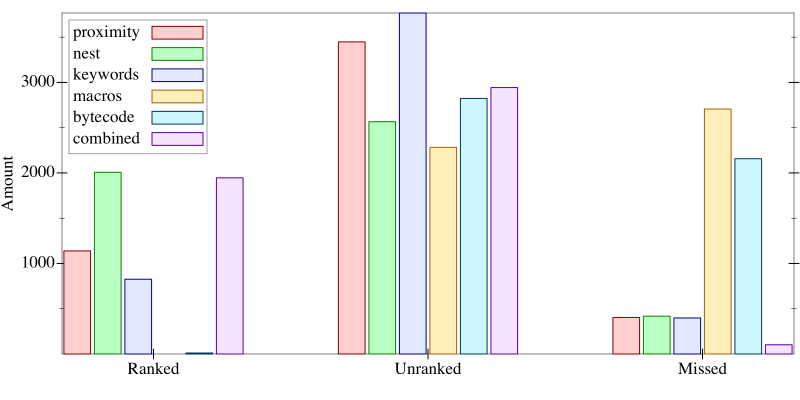
\includegraphics[width=1.0\textwidth]{../output/synthesis/ranker/Remove-combined.png}
\caption{Ranking results. Ranked refers to completions in the top five positions. Missed means they weren't in the results at all.}
\label{fig:ranker-combined}
\end{figure}

\begin{figure}[h]
\centering
\hrule
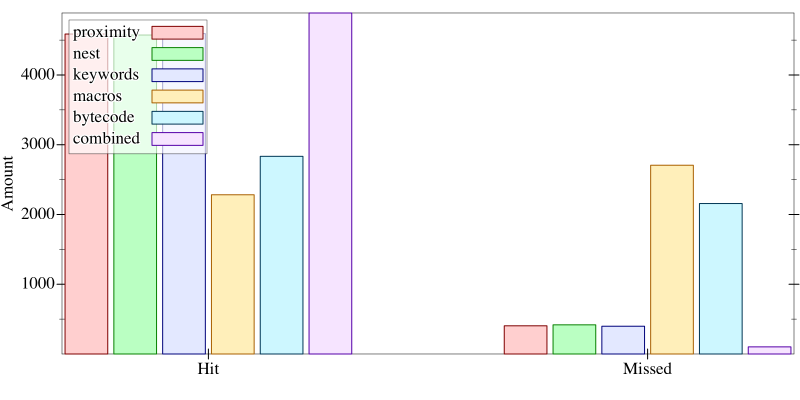
\includegraphics[width=1.0\textwidth]{../output/synthesis/ranker/Remove-uber-combined.png}
\caption{Pass/fail ranking results}
\label{fig:ranker-uber-combined}
\end{figure}

Figure~\ref{fig:ranker-combined} shows the results of the ranker.
The ranked section shows how many tokens appeared in the top five suggestions for each method.
The unranked section shows how many tokens were suggested anywhere in the list.
The missed section shows how many tokens did not appear in the completion suggestions at all.
Figure~\ref{fig:ranker-uber-combined} shows the same data, but combines the ranked and unranked sections into one hit section, focusing more on existence rather than order.

Looking at the methods individually, the textual methods did a much better job than the macro methods at not only including expected tokens in the list of results, but also prioritizing them well.
Even though macro heuristics and analysis suggested many of the correct tokens, almost none of the results were in the top five positions.
This is mainly because textual heuristics are done on the source code, making different ordering algorithms easy to experiment with and use.
On the other hand, macro heuristics and analysis are more meta by nature, not lending themselves to obvious sorting algorithms, leaving alphabetical the main alternative.

Among the textual methods, sorting by nesting level was by far the most effective.
Of the tokens that correctly made it into the list of results, nearly 45\% of them were ranked in the top five, as opposed to less than 25\% for the other two textual methods.

Of the macro methods, macro analysis did roughly 25\% better than macro heuristics.
This makes sense as macro analysis is actually compiling the code to get fully expanded macros as well as all external dependencies.
However, the fact that macro heuristics did so well in comparison makes it a good fallback for when the code is in an uncompilable state.

It is also interesting to note that truncating the text (as opposed to simply removing the token) adversely affected the textual methods as expected, but the macro methods were barely affected at all.

Since macro analysis did better in the macro camp and nesting level did better in the textual camp, we decided to combine the two.
Nesting level did much better at ordering, so those results were ordered first, with macro analysis results appended.
The results were that the results showing up in the top five spots stayed about the same, whereas the results that didn't show up at all were decreased by about 75\%.
This shows that the results provided by the two methods were significantly non-overlapping.

\section{Checker Results}

\begin{figure}[h]
\centering
\hrule
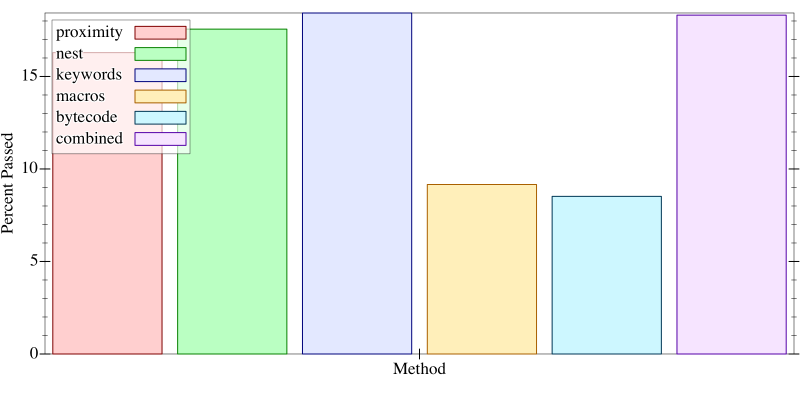
\includegraphics[width=1.0\textwidth]{../output/synthesis/checker/Remove-Percent.png}
\caption{Percent of checker runs without errors using the token removal source alteration method.}
\label{fig:checker-remove-percent}
\end{figure}

\begin{figure}[h]
\centering
\hrule
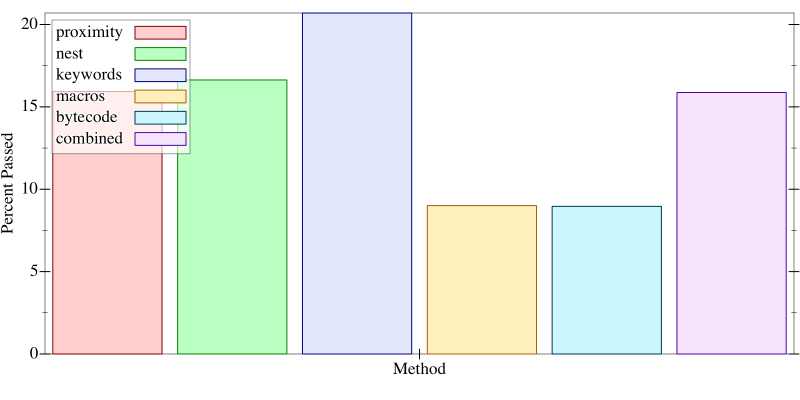
\includegraphics[width=1.0\textwidth]{../output/synthesis/checker/Truncate-Percent.png}
\caption{Percent of checker runs without errors using the file truncate source alteration method.}
\label{fig:checker-truncate-percent}
\end{figure}

Each original source token removed results in a list of completion suggestions.
The checker replaces the token with a single suggestion and runs the resulting new program.
If the program compiles and runs to completion without exceptions, the completion is considered a success.
Otherwise, the run is marked as a failure.

Figure~\ref{fig:checker-remove-percent} shows the percent of successful runs for each completion method when the removal source alteration method was used to modify the original source.
Figure~\ref{fig:checker-truncate-percent} shows the same data, but for completions suggested after using the truncate source alteration method.

Because the checker checks the first five results for success or failure, it is expected that the success rate of the checker would to a certain degree follow the success rate of the ranker.
Therefore, it is not surprising that the textual methods had a higher success rate than the macro methods.

It is interesting to note that, among the textual methods, the function keywords approach led to the least failures.
This makes sense because it is not unlikely to have multiple functions that take the same number and type of arguments, thus allowing the program to run without crashing (although likely with incorrect end results).

The type of the top occurring error for each method is also instructive.
For the textual methods, the top occurring error by far is using unbound identifiers.
This makes sense because the completer is using every token in the file to present completion results, and many of them will not be bound at all or will be bound in a local context.
The function keywords approach had the least percentage of unbound identifier failures (28\% as opposed to 32\% and 34\%), which makes sense because functions are often defined at the top level, making them available anywhere in the module.

For the macro methods, the top occurring errors were syntax errors, which happened about twice as much as unbound identifier errors.
This is instructive and expected because the point of the macro methods is to bring in globally available identifiers from external sources such as ones provided by the language itself or by imported modules, so incorrect use of them is most likely to be syntax related.

The results didn't show much difference between removing tokens and truncating the file as far as failures go.
The one interesting thing to note is that the success percentage actually went up by truncating text for the function keywords method.
This could mean that because the truncated file had fewer functions to choose from, the likelihood that one of them would match the calling function signature would be higher.
However, it also suggests that functions are generally used after the definition, so truncating later functions tends to prune the number of incorrect functions.

\section{Summary}

The purpose of the testing framework is to provide useful information about specific completion implementations.
Implementing and analyzing several completion methods serves to validate the testing framework.

Some things we discovered about the completion methods from running the testing framework include:

\begin{itemize}

\item Textual methods performed better than macro methods in general.
\item Completions from textual methods and macro methods were largely non-overlapping.
\item Combining methods improved results
\item Results degraded with the truncate source alteration method.

\end{itemize}

Without a testing framework to test completion methods against, this information would be guesswork.

\chapter{Conclusions}

There is little to no formal testing of auto-completion systems in the literature.
Without testing frameworks such as the one implemented in this thesis, knowing how well the completer performs and what improvements will give the best results is hard at best, requiring user studies or user feedback from actual users.
To show the value a testing framework can provide, we ran different completion methods against the testing framework and compared the results to our initial hypotheses about the relative value of the methods.

Our initial guess was that textual heuristics would be the least useful, and that structural heuristics and macro heuristics/analysis would be equally better than textual heuristics.
By analyzing the results of the testing framework, we realize that macro heuristics/analysis is significantly worse than the textual methods, and that textual heuristics only performed slightly worse than structural heuristics.
This data can help lead to the important conclusion that most tokens used are already somewhere else in the same source file.
This conclusion can then lead to more informed decisions about how best to improve the completer and its results.

Although macro heuristics/analysis performed significantly worse on their own than textual methods, we were correct in assuming that combining the two methods would give better results.
Analyzing the data from the testing framework also helped reveal the fact that, although macro methods didn't do extremely well on their own, the subset of completions they provide is significantly non-overlapping to the subset of completions the textual methods provide.
By combining the best of both categories, the number of tokens that simply didn't appear in the completion list was reduced by a significant 75\%.

Comparing the results of the ranking part of the test framework to the error checking part can also lead to making informed decisions based on the priorities of the completer.
For instance, while the nesting method performed better at ranking results, the function keyword method did better at not suggesting failing results.
Different priorities can lead to different informed decisions about where to invest resources.

In general, we found that the data provided by a testing framework is valuable data that can lead to making more informed decisions about the direction of the completion system.
Although user testing and resulting feedback is very valuable, having an automated testing framework can be invaluable in making early informed decisions that can save time and money.

\section{Future Work}

The testing framework collects a significant amount of raw data, but for the most part this data must be synthesized and displayed manually.
It is probable that certain data from the set would be more useful in improving and iterating on completion systems.
As these data patterns arise, it would make sense for the testing framework to automatically extract and conveniently display this data every run.

The macro heuristics and analysis methods barely scratched the surface of what information is available because of the power and complexity of the macro system.
Although the macro heuristics method finds the most common macro patterns, there are many others that are ignored that may provide differing returns depending on the code the method is run on.

The most beneficial work for the completers would probably come from improving the macro analysis method by gleaning more information from the bytecode.
The bytecode has all of the information necessary to run the program, giving opportunity for more sophisticated methods of extracting and ordering the available completions.

\bibliographystyle{plainnat}
\bibliography{bib}

\end{document}

% vim: lbr
